\appendix
\section*{\Huge Supplemental Material}

\setcounter{section}{0}

% https://tex.stackexchange.com/a/708552/316176
\makeatletter
\def\@seccntformat#1{\@ifundefined{#1@cntformat}%
   {\csname the#1\endcsname\space}%    default
   {\csname #1@cntformat\endcsname}}%  enable individual control
\newcommand\section@cntformat{\thesection.\space} % section-level
\makeatother
\renewcommand{\thesection}{S\arabic{section}}
\counterwithin{equation}{section}
\counterwithin{figure}{section}
\counterwithin{table}{section}
\counterwithin{theorem}{section}
\counterwithin{algorithm}{section}
\counterwithin{lstlisting}{section}

\vspace{0.8em}

Below is supplemental material for our paper TODO with discussions and figures that were not put in the main paper.

\subsection{Algorithm Equivalency}

\label{sec:algorithm:equivalency}

We shall demonstrate the accuracy of the proposed shortcut algorithm by providing a proof overview of how it is equivalent to the old algorithm (and assuming the old algorithm is a `good' reconstruction algorithm).
We define `equivalent' in this context to mean that every node at which an organism can be placed by the naive algorithm is also a node at which one can be placed by the shortcut algorithm (i.e. the shortcut algorithm places nodes at points that the naive algorithm could, given the right arbitrary choices).

Consider adding some organism $o$ to the reconstructed tree $T$, which follows exactly one of the following cases: there is no missing information (i.e. $\forall (r, d) \in o\ r = \operatorname{rank}(\operatorname{children}(n))$, where $n$ is the current node throughout iteration), or there is.
The case where there is no missing information is trivial -- the only difference between the original and new algorithm lies when there is missing information, the absence of which rendering them the same.

Therefore, consider analyzing data at rank $r$ and having some missing information between the $\operatorname{rank}(n)$ and $r$.
Now, consider cases on whether there is some successive path of matching differentiae:

\begin{itemize}
  \item \textbf{There is some path.}
  Therefore, we know that this path contains a descendant $n'$ of $n$ with rank $r$ and differentia $d$.
  In the naive algorithm, this descendant is select to be the next $n$ when processing the information of $o$, as the optimal path found includes $n'$.
  However, we also know that the shortcut algorithm must have created a shortcut from $n$ to $n'$ (and possibly collapsed it with other valid descendants, which is irrelevant as the path still remains).
  So, the shortcut algorithm (in line 10 of the naive Algorithm~\ref{alg:old} as described in the paper) finds this child and selects it to be the new $n$ as well.
  \item \textbf{There is no such path.}
  Since there is no candidate path to follow, the naive algorithm simply creates a new node branching off $n$ with rank and differentia $(r, d)$.
  Then, this new node is made the new $n$.
  Since there was no valid path, we see that $n$ has no descendants with rank $r$ and differentia $d$.
  Therefore, there is no shortcut built from $n$ to such a node, as it does not exist.
  So, the shortcut algorithm will also branch off of $n$ by creating a new node in the same manner as the naive one.
\end{itemize}

In either case, we have shown that both algorithms make effectively the same decisions when it comes to selecting nodes $n$ throughout each iteration of \textsc{TreeInsert}.
Because original relationships between nodes are still preserved, choosing a particular node to branch off of conveys identical information in both algorithms.
In conclusion, the two algorithms are equivalent in correctness.
However, it is worth noting that in cases where multiple paths are valid, the algorithms may make different decisions (as the chosen path out of these is arbitrary) and therefore may not be exactly equivalent.

\subsection{Validation with Ground Truth}

In addition to determining triplet distance between ground truth and reconstructed phylogenies, we ran visualizations to make comparisons more interpretable.

\begin{figure}[h]
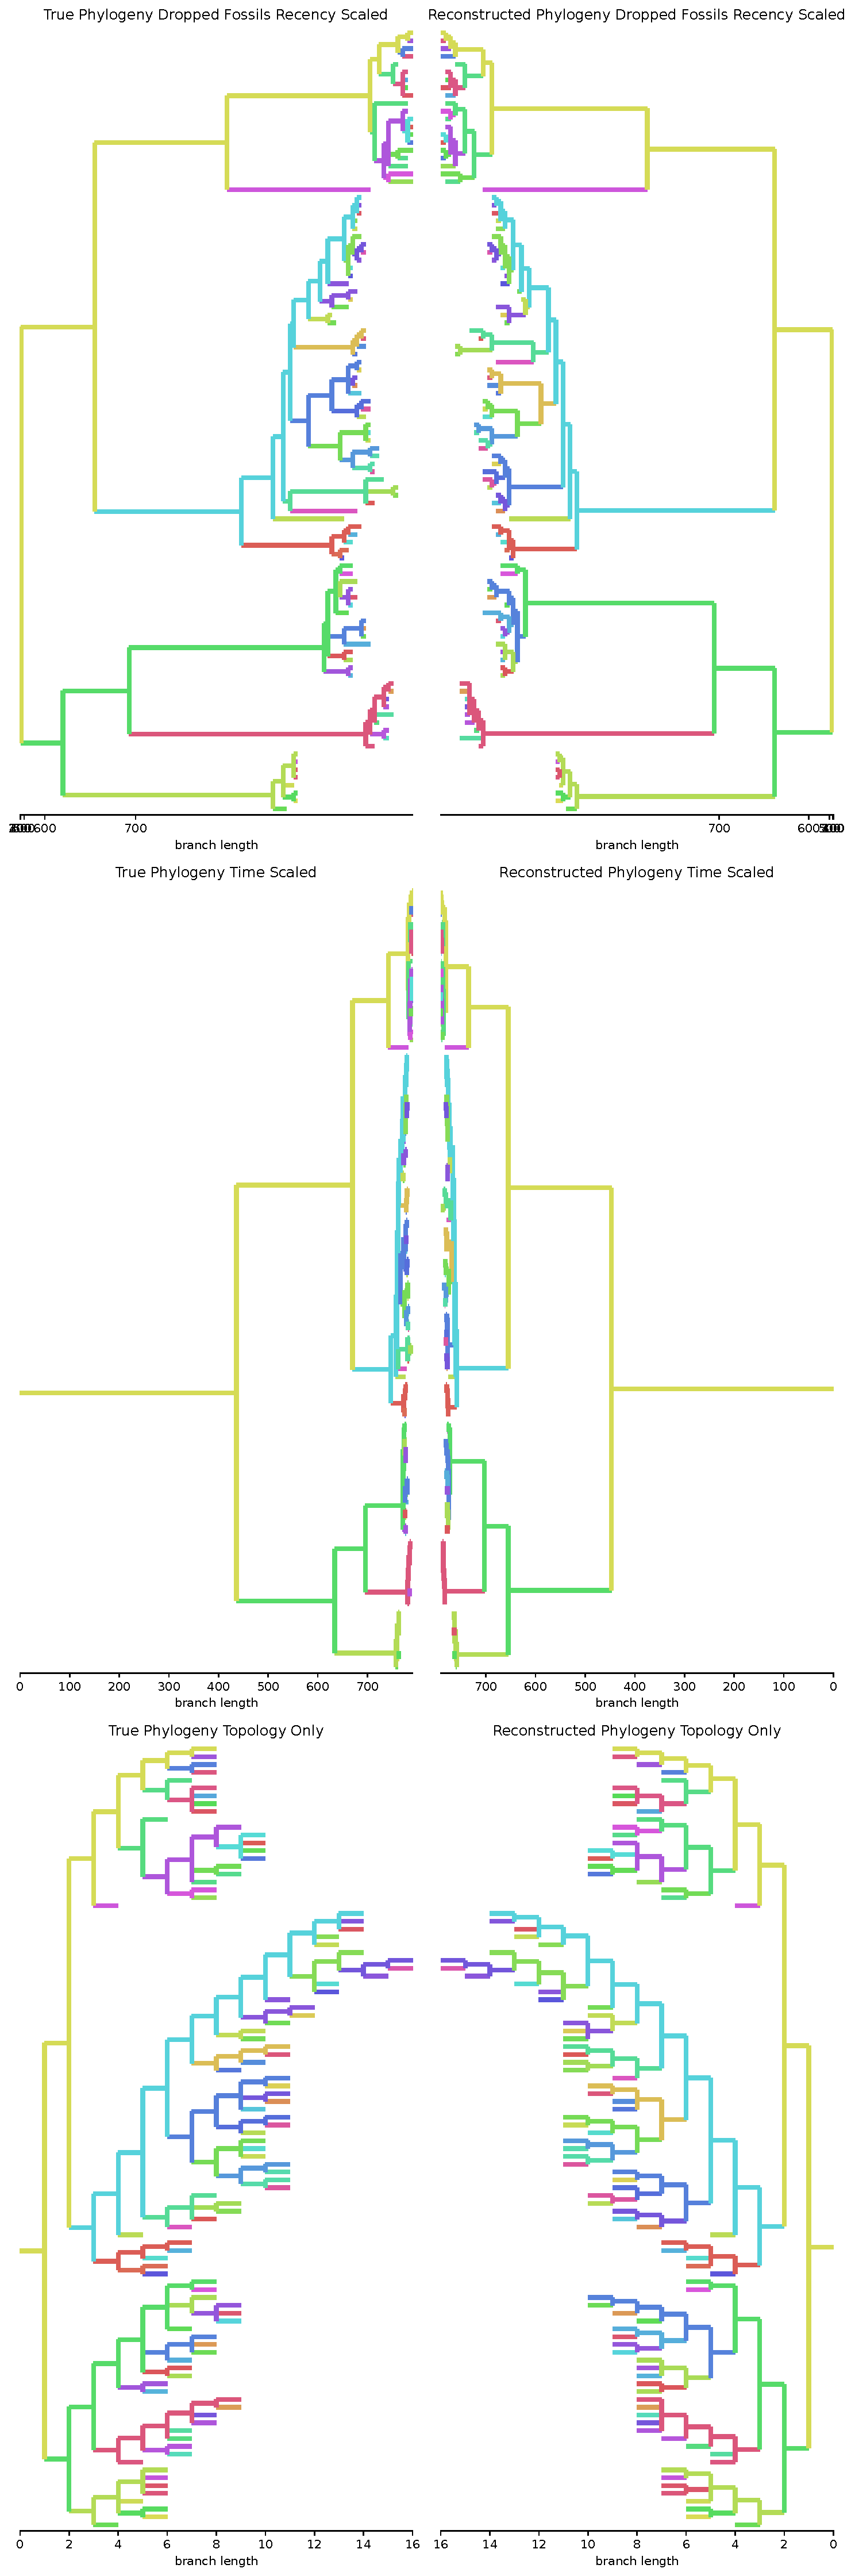
\includegraphics[width=\columnwidth,trim={0 52cm 0 0.8cm},clip]{img/colorclade.pdf}
\caption{\textbf{Sample comparison of true and reconstructed phylogenies.}
\small
Generated using a tilted retention policy and a surface of 32 bits. The true phylogeny is on the left and the reconstructed phylogeny is on the right. Colors are based on a hash from the taxon label for each tip to better facilitate visual comparison. Reconstruction error for this reconstruction was 2.6\%. Visualization created with colorclade \citep{moreno2024colorclade}.
}
\label{fig:colorclade}
\end{figure}

